\documentclass{article}
\usepackage[T1] {fontenc}
\usepackage[italian]{babel}
% Per i link nell'indice
\usepackage{hyperref}
\usepackage{cite}
\usepackage{graphicx}
\graphicspath{ {./images/} }

\title{Lezioni sul Moto Armonico}
\author{Matteo Savatteri}

\begin{document}
\maketitle

\tableofcontents

\section{Introduzione}
Questo documento presenta un ciclo di lezioni sul moto
armonico, indirizzate a una classe 4\textsuperscript{a}
di liceo scientifico italiano e preparate secondo il
\emph{Modello di Istruzione 5E} \cite{bybee2009bscs}.
Questo metodo di natura inquiry prevede cinque fasi:
\emph{Engage}, \emph{Explore},
\emph{Explain}, \emph{Extend}, \emph{Evaluate}.

\section{Engage}
Per far scoprire ai ragazzi l'esistenza del moto armonico e
la sua descrizione, occorre innanzitutto attirare la loro
attenzione portando in classe un sistema che mostri un moto
oscillatorio. A questo scopo mostro agli studenti un modellino di
\emph{pendulum wave} (Figura \ref{fig:pendulum_wave}):
serie di pendoli agganciati a un sostegno in legno mobile.
Ciascun pendolo è costituito da un filo di stessa lunghezza
e da un pesetto di uguale massa. 
Faccio oscillare contemporaneamente tutti i pendoli:
tutti hanno lo stesso periodo. 
Modifico la lunghezza dei pendoli sollevando un'estremità del
sostegno e li faccio oscillare contemporaneamente. I periodi
dei diversi pendoli si modificano in modo che si formi un'onda
longitudinale (guardando il sistema dall'alto).

\begin{figure}
\centering
  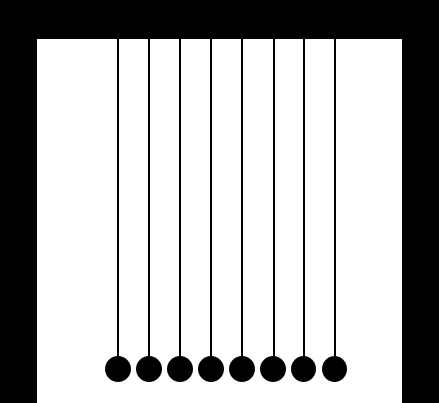
\includegraphics[width=0.32\textwidth]{image3}
  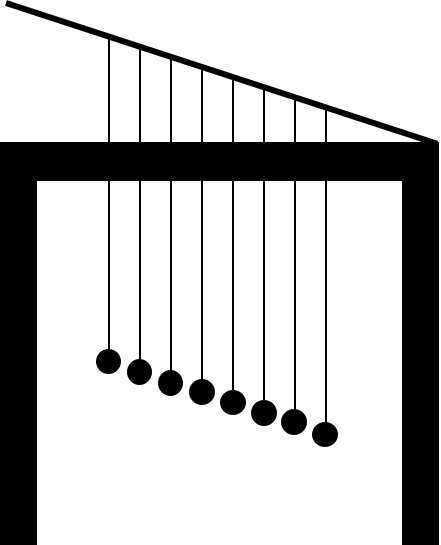
\includegraphics[width=0.32\textwidth]{image2}
  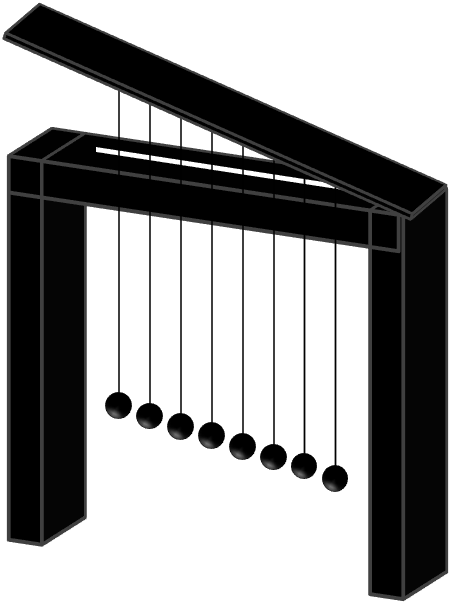
\includegraphics[width=0.32\textwidth]{image1}
  \caption{Modello di pendulum wave}
  \label{fig:pendulum_wave}
\end{figure}

\section{Explore}
In questa fase si chiede agli studenti di dividersi a gruppi di tre
o quattro e di eseguire un compito un po' più difficile: scegliere
3 dei fenomeni presentati nella fase di engage e disegnare i
grafici della forza a cui sono sogetti i corpi in funzione della
loro traiettoria. Per facilitare questo compito conviene
scegliere un sistema di riferimento avente asse curvilineo
e coincidente con la traiettoria dei moti esaminati e graficare
la proiezione della forza su tale asse. Si noti che questo
esercizio non richiede di conoscere la natura delle forze in
gioco \cite{barbieri2015good}.

\section{Explain}
Nella lezione seguente si può approcciare la fase di explain.
Essa dovrebbe essere svolta sotto la guida dell'insegnante e 
sulla base dell'esperienza che gli studenti hanno acquisito nelle
fasi precedenti. E fondamentale che a questo punto gli studenti
condividano le spiegazioni dei fenomeni che essi stessi
hanno sviluppato \cite{duran20045e}.

In questa fase l'obbiettivo è arrivare a comprendere che
un corpo si muove di moto armonico se per le sue piccole
oscillazioni la relazione forza-posizione è della forma:

\begin{equation}
F_{\zeta}=-k\zeta, \quad k>0
\end{equation}

Dove $\zeta$ è una coordinata curvilinea. 

Il professore si può avvalere del software
\emph{tracker}\footnote{\url{https://physlets.org/tracker/}}
per mostare agli studenti gli effettivi grafici forza-posizione
degli esperimenti di interesse.

\section{Extend}
Ora lo studente è pronto a mettere in pratica le conoscenze
acquisite, estendendo la sua comprensione dell'argomento
sulla base di esse. Una competenza molto utile da acquisire
è quella di riconoscere l'armonicità di un moto, basandosi
semplicemente sull'osservazione del fenomeno.

Un corpo oscilla armonicamente nell'intorno di un punto
di equiibrio solo se \cite{giliberti2014detecting}:

\begin{itemize}
\item Il punto di equilibrio $\zeta=0$ è \emph{stabile};
\item La funzione $F_{\zeta}$ è continua;
\item La funzione $F_{\zeta}$ è differenziabile;
\item $\frac{\mathrm{d}F_{\zeta}}{\mathrm{d}\zeta}(0) \neq 0$
\end{itemize}

Da queste considerazioni si può dedurre che un moto
è armonico se ha un punto di equilibrio e se appare
\emph{liscio} e \emph{isocrono}.
Esiste trucco che permette di verificare l'isocronia
nel caso di alcuni moti: ascoltare il rumore prodotto
dal moto e verificare che la sua frequenza non cambia al
variare dell'ampiezza delle oscillazioni.

In questa lezione si propone di portare gli studenti
in laboratorio, dove si divideranno a gruppi di tre
o quattro studenti proveranno a progettare un esperimento
che mostri l'armonicità o l'anarmonicità di un certo moto.
Gli studenti dovranno avvalersi di strumenti di misura,
come cronometro e metro, per valutare l'isocronia del
moto scelto.

\section{Evaluate}
\underline{TODO}

\bibliography{bibliografia}{}
\bibliographystyle{plain}

\end{document}
